\documentclass[masters]{ucbthesis}
\usepackage{biblatex}
\usepackage{graphicx}
\usepackage{subcaption}
\usepackage{amsmath}
\usepackage{capt-of}
\usepackage[bottom]{footmisc}
% Double spacing, if you want it.
% \def\dsp{\def\baselinestretch{2.0}\large\normalsize}
% \dsp

% If the Grad. Division insists that the first paragraph of a section
% be indented (like the others), then include this line:
% \usepackage{indentfirst}

\newtheorem{theorem}{Jibberish}

\bibliography{references}

\hyphenation{mar-gin-al-ia}
\hyphenation{bra-va-do}

\begin{document}

% Declarations for Front Matter

\title{Deep Networks for Equalization in Communications}
\author{Laura Brink}
\degreesemester{Fall}
\degreeyear{2018}
\degree{Master's of Science}
\chair{Professor Anant Sahai}
\othermembers{Professor John Wawrzynek}
\numberofmembers{2}
% Previous degrees are no longer to be listed on the title page.
% \prevdegrees{B.A. (University of Northern South Dakota at Hoople) 1978 \\
%   M.S. (Ed's School of Quantum Mechanics and Muffler Repair) 1989}
\field{Electrical Engineering and Computer Science}
\campus{Berkeley}

% For a masters thesis, uncomment (remove the % at the beginning of)
% the following line.  This affects the title and approval pages,
% which by default calls this a "dissertation", not a "thesis".

%\itsamasters

% The title page generated by LaTeX is now acceptable for handing in.
% (This was not always the case).

\maketitle
\approvalpage
\copyrightpage

% (This is included by thesis.tex; you do not latex it by itself.)

\begin{abstract}

% The text of the abstract goes here.  If you need to use a \section
% command you will need to use \section*, \subsection*, etc. so that
% you don't get any numbering.  You probably won't be using any of
% these commands in the abstract anyway.

We apply the techniques from meta-learning and machine learning to the communications domain.  
Specifically, we explore how neural networks can learn to equalize new channel environments without training on them and how neural networks can learn to estimate and correct carrier frequency offset for new rates of rotation without training on them.  
We show that deep neural networks can learn to learn to estimate channel taps for two tap channels.
We also explore how deep recursive neural networks learn to learn to equalize for any given channel.  
We demonstrate that neural networks can learn to learn to estimate and correct carrier frequency offset for new rates of rotation.  Crucially, we do all of this without using backpropagation to re-train the networks for each new set of environmental conditions.

\end{abstract}


\begin{frontmatter}

%\begin{dedication}
%\null\vfil
%\begin{center}
%To J
%\end{center}
%\vfil\null
%\end{dedication}

\maxtocdepth{subsection}
\tableofcontents
\clearpage
\listoffigures
%\clearpage
%\listoftables

%\begin{acknowledgements}
%I want to thank my advisor for advising me.

%\end{acknowledgements}

\end{frontmatter}

\pagestyle{headings}

% (Optional) \part{First Part}


With the rise of internet of things, more and more users will need to access the wireless spectrum.  As the spectrum becomes saturated with users, not only must our systems adapt to changing environments but also be able to coexist and thrive in the presence of unknown neighbors.  
We must design a robust communications system that will give us the freedom to. 

Most communications systems have three main processes; equalization, demodulation, and error-correction.  While we will need to design robust forms of all of these processes, we will focus on equalization for the remainder of this paper. 


\subsection{Inter-symbol Interference and Equalization}

What is equalization and ISI? 

Inter-symbol interference occurs when we are transmitting over a channel that has some echos.  These echos cause the receiver to hear a garbled signal instead of the original signal from the transmitter.  This is called inter-symbol interference because the receiver is hearing a combination of symbols across time. 

Let $\vec{x}=[x_0, x_1, \ldots x_n]$ be the set of $n$ complex symbols that the transmitter sends over the channel that connects the transmitter to the receiver.
Each channel will have different characteristics. Some channels may have echos, others may have delays, often channels will have both.  When a channel has echos, this is called a multipath channel because there are multiple paths to reach the receiver.  Each path is called a tap.  We can characterize a channel by characterizing the taps.

What can cause these echos?  How prevelant are they?

Channel taps:
Let $\vec{a} = [a_0, a_1, \ldots a_l]$ be the set of characteristic for a multipath channel that has $l$ taps. When a sequence of symbols like $\vec{x}$ is transmitted over this channel, the channel taps are convolved over the sequence.  Additionally, there is noise in the system denoted by $\eta_i$. 

$$\tilde{x}_m = \sum_{i=0}^l a_i x_{m-i} + \eta_i$$

The receiver will hear a signal that is corrupted by inter-symbol interfence and noise;
$\tilde{\vec{x}}=[\tilde{x}_0, \tilde{x_1}, \ldots \tilde{x}_{n+l}]$. 

Receivers must be able to handle garbled signals in order to transmit data in the real world.  The process of removing the inter-symbol interference is called equalization.  The goal of equalization is to take in a garbled signal and output a signal without any inter-symbol interference. 

INSERT IMAGE OF 2 TAP CHANNEL EFFECTS ON QPSK

Engineers have built processes to remove inter-symbol interference.  First, let's go into the case when the channel characteristics are known.

\subsubsection{Equalization for a known channel}
If you know the channel characteristics, $\vec{a}$, perfectly, then there are a few different methods that can be used. 

Zero-forcing

While it's important to consider how well a receiver can equalize with a known channel, this is rarely the case.  Usually, we do not know the channel characteristics.

\subsubsection{Equalization for an unknown channel}
When the receiver does not know the channel characteristics, the process of equalization essentially has two jobs; first, identify the channel, second, remove the inter-symbol interference. If the receiver did not identify the channel first, there would be no way to remove the affects of it on the received signal. 

In order to do channel estimation, most systems require that packets begin with a known sequence called a preamble. 

Channel estimation: least squares

Minimum mean squared error equalizer.
 
\subsubsection{How do real systems handle equalization?}

OFDM does not have this problem!

 
\subsection{Carrier Frequency Offset and Correction}

Now, if we were to implement our minimum mean squared error algorithm on a physical receiver, we would find some problems with our equalization process.  
Our equalizer will equalize the first symbols very well.  However, as we equalize end parts of our sequence, we will encounter a physical phenomonen called carrier frequency offset, CFO.

Carrier frequency offset occurs when ???

When there is a significant CFO present, our symbols will gradually start rotating. CFO will effect our received symbols like

$$\tilde{x}_m = x_m e^{mj\omega}$$


The effect will look like something like this 

INSERT IMAGE OF CFO OCCURRING on QPSK

\subsubsection{How do real systems handle CFO correction?}

There are a few ways to handle CFO, some are more elegant than others. 

The first solution is to try to remove the problem.  Since CFO is dependent on the length of a packet, one solution is to make packets so short that 

A more elegant solution is using phase-lock loops (costas loops).

What must a modern day receiver handle?  What does it look like when we have both CFO and ISI?

$$\tilde{x}_m = (\sum_{i=0}^l a_i x_{m-i})e^{mj\omega} + \eta_i$$

INSERT IMAGE OF AFFECTS OF BOTH CFO AND EQUALIZATION

INSERT IMAGE OF SAME THING WITH NOISE!

\subsection{Replicate Results}

\subsection{Channel Estimation}

\begin{itemize}
\item compare least squares and how KNN did with pure deep nn based architecture
\item NN did better than least squares
\item hyperparam search over general 1-layer to 4-layer dense layers, and number of nodes and activations
\item plots: how error changed with respect to data points, as number of data points increased, NN outperformed LS
\item preamble: 100
\item want: QPSK, plot of preamble length
\item want? how to visualize that NN does better than LS
\end{itemize}

\subsection{Channel Equalization}

\begin{itemize}
\item compare to MMSE
\item re run with the new RNN architecture
\item backprop length of ~ 3. crude search from 1-10. 2 tap channel
\item added channel preprocessing: didn't seem to make too much of a difference
\item plot log/ log scale to find converging in error
\end{itemize}

\subsubsection{Learning an inverse}
\begin{itemize}
\item can a NN learn to do division?
\item given a one tap channel and data sequence, output is equalized data sequence
\item with and without log feature scaling
\item without log errors = $10^-6$
\item MMSE gets error = $10^-32$
\item with log errors = 
\item straight inversion, without log feature scaling $10^-7$ - with dense layers
\item inversion with log feature scaling with error of $10^-14$ 
\item plots: inversion, but as a function of beta for both non-log and log
\end{itemize}

\subsubsection{Learning to multiply two inputs}
NN given x, y - output x*y

\subsection{Channel Est + Equal}
re run that 
\chapter[Deep Networks for Carrier Frequency Offset]{Deep Networks for Carrier Frequency Offset\raisebox{.3\baselineskip}{\normalsize\footnotemark}}
\footnotetext{The contents of this chapter were produced in collaboration with Nikhil Shinde, an undergraduate researcher that I am mentoring.} 

The carrier frequency offset (CFO) correction process removes the symbol rotation caused by the non-ideal conditions of the transmitter and receiver environment.  We will explore how neural networks can both estimate the CFO and correct for the rate of rotation without using backpropagation for each new rate.

\section{Recurrent Neural Network Follows a Circle}

A carrier frequency offset affects the received symbols by slowly rotating them around the origin.  If we want a neural network to be able to correct this, we essentially need it to act as a clock, following around a circle at a certain rate.
We first explore what kind of architectures are necessary for a recurrent neural network (RNN) to learn how to follow a circle.
We show that a simple, small linear RNN can learn to act as the rotation matrix for a single rate of rotation around a circle.
We also show that in order to have an RNN follow a circle for different rates of rotation, we need a large non-linear layer.
We will then design a deep neural network to estimate the rate of rotation caused by CFO and correct it.

\subsection{Single Rate}

Figure~\ref{fig:circle_constant_rate} shows a recurrent neural network (RNN) that follows a circle for a single rate of rotation.  The network's input is the starting point, $x_0$, and it must predict the next $99$ points, $x_1 \ldots x_{99}$.  Point $x_m$ is rotated by $e^{mj\omega}$ where $\omega$ is the rate of rotation.  The RNN architecture is one linear layer that takes the current point as input, $x_m$, and outputs the next point, $x_{m+1}$.  We are forcing the state of the RNN to be the estimate of the next point; $\text{state} = \hat{x}_{m+1}$.  We use a linear layer here because the network essentially has to learn how to become the rotation matrix which is linear with respect to the input. 

\begin{align}
R = \begin{bmatrix}
\cos(\omega) & - \sin(\omega) \\
\sin(\omega) & \cos(\omega)
\end{bmatrix}
\end{align} 

\setlength{\tabcolsep}{0pt}
\begin{figure}
  \centering
  \caption{Linear neural network: follow a circle for a constant CFO rate, $\omega=0.02$. The figure on the left shows the original data of length $100$. The figure in the middle shows the estimated data from the neural network given the starting point from the left figure.  The figure on the right shows the log of the test cost of the neural network versus traing epoch.}
  \begin{tabular}{ccc}
    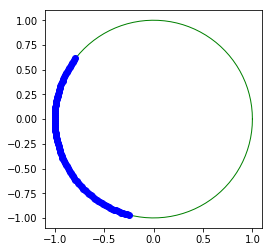
\includegraphics[width=50mm]{figures/cfo/follow_circle_linear_before.png}&
    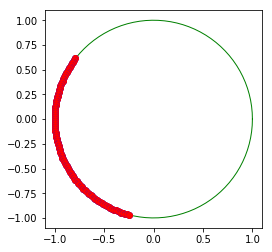
\includegraphics[width=50mm]{figures/cfo/follow_circle_linear_after.png}&
    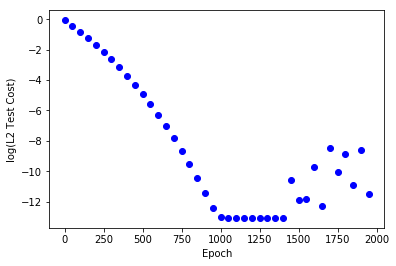
\includegraphics[width=70mm]{figures/cfo/follow_circle_linear_loss.png}\\
  \end{tabular}
  \label{fig:circle_constant_rate}
\end{figure}

The RNN is trained for a constant rate of rotation, $\omega$, applied to sequences of $100$ points.  The network trained for $2k$ epochs, each with a batch size of $1k$ data sequences and with a learning rate of $0.006$.  The initial starting point, $x_0$ is a uniform random variable drawn from on the unit circle. 
The network is tested on $1k$ new data sequences but with the same $\omega$.
Figure~\ref{fig:circle_constant_rate} shows the results of an RNN trained and tested for $\omega=0.02$.  
The network achieves a loss on the order of $10^{-13}$.  However, the minimum loss is not very sticky.  Notice that the figure on the right in figure~\ref{fig:circle_constant_rate} shows the network jumping away from this minimum while training at around $1400$ epochs.  A more thorough search over learning rate decay is needed to prevent this jumping from happening.

\subsection{Different Rates}


Figure~\ref{fig:circle_diff_rate} shows a recurrent neural network (RNN) that follows a circle for a given rate of rotation.
The network's inputs are the starting point, $x_0$ and the rate of rotation, $\omega$.
The RNN must predict the next $99$ points, $x_1 \ldots x_{99}$.  Point $x_m$ is rotated by $e^{mj\omega}$.

\setlength{\tabcolsep}{0pt}
\begin{figure}
  \centering
  \caption{Nonlinear neural network: follow a circle for different CFO rates. The figure on the left shows the original data of length $100$ for $\omega=0.01063284$. The figure in the middle shows the estimated data from the neural network given the starting point and rate of rotation from the left figure.  The figure on the right shows the log of the test cost of the neural network versus traing epoch.}
  \begin{tabular}{ccc}
    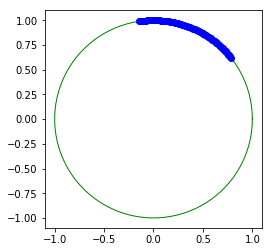
\includegraphics[width=50mm]{figures/cfo/follow_circle_nonlinear_before.png}&
    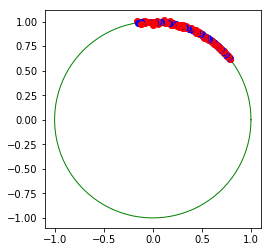
\includegraphics[width=50mm]{figures/cfo/follow_circle_nonlinear_after.png}&
    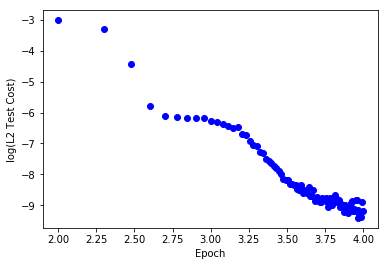
\includegraphics[width=70mm]{figures/cfo/follow_circle_nonlinear_loss.png}\\
  \end{tabular}
  \label{fig:circle_diff_rate}
\end{figure}

We cannot use just linear layers in this case because the RNN must learn to find $\cos(\omega)$ and $\sin(\omega)$ for different $\omega$.  Essentially, this RNN needs to approximate the $\sin, \cos$ functions and then apply them to the state.

The RNN architecture consists of one non-linear layer, with $100$ nodes and Relu activation functions, and a linear layer at the output with $2$ nodes. The inputs to the RNN are the estimated current point, $\hat{x}_m$, and the rate of rotation, $\omega$.  The RNN outputs the estimate of the next point, $\hat{x}_{m+1}$.  We are forcing the state of the RNN to be the estimate of the next point concatenated with the rate of rotation; $\text{state} = [\hat{x}_{m+1},\omega]$ so that state then becomes the input to the next run of the RNN.

The RNN is trained for different rates of rotation, $\omega$, applied to sequences of $100$ points.
The rate of rotation is a uniform random variable $[0,\frac{1}{50}]$.
We use mean squared error of the true data sequence and the estimated data sequence for the loss function; $||\vec{x}-\vec{\hat{x}}||^2$.  The network is trained for $10k$ epochs, each with a batch size of $1k$ data sequences and with a learning rate of $0.01$.  The initial starting point, $x_0$ is a uniform random variable drawn from on the unit circle.
The network is tested on $100k$ new data sequences with random $\omega$.
Figure~\ref{fig:circle_diff_rate} shows the results of an RNN trained and tested for $10k$ epochs.  The network achieves a loss on the order of $10^{-5}$ but is still data hungry and should be trained for more epochs.


\section{Deep Network Carrier Frequency Offset Estimation and Correction}

We explore estimating carrier frequency offset and correction with neural networks.
One of the challenges with CFO is that it cannot be directly measured in the real world.  
Therefore, all of the loss functions will not depend on $\omega$.
Again, we want a neural network that does not need to update its weights every time it encounters a new rate of rotation.

The inputs of the neural network are the known preamble, $\vec{x}_{pre}$, and the received preamble, $\vec{\tilde{x}}_{pre}$.  The neural network outputs the estimated preamble symbols, $\vec{\hat{x}}_{pre}$.  
The loss function is the mean squared error between the original preamble and the estimated preamble, $||\vec{x}_{pre}-\vec{\hat{x}}_{pre}||^2$.
The neural network architecture consists of two non-linear layers, each with $10$ nodes and sigmoid activations.  This then feeds into a linear layer that outputs a scalar, treated as the estimate for the rate of rotation, $\hat{\omega}$. 
The received preamble is then rotated using a special layer with the function $e^{-mj\hat{\omega}}$ that is differentiable and can pass gradients.

Figure~\ref{fig:cfo_est} compares the performance of the neural network correcting CFO versus no CFO correction.  The training and testing data are solely for a one tap channel and have varying values of $\omega$. The preamble length is kept constant at $100$ symbols in QPSK.
The neural network is trained for $15k$ epochs with batch size of $100$ sequences and with a learning rate of $0.001$.  The neural network and no CFO correction are tested on $10k$ sequences with different rates of rotation, $\omega$.  
The rate of rotation, $\omega$, is a uniform random variable, $[0,\frac{1}{100}]$.
The training and testing process is repeated for each SNR.  Note, we re-train the network for each SNR.  
We compare the bit error rate of the neural network and classic demodulator versus the bit error rate of just the classic demodulator without any CFO correction.

\begin{figure}
\begin{center}
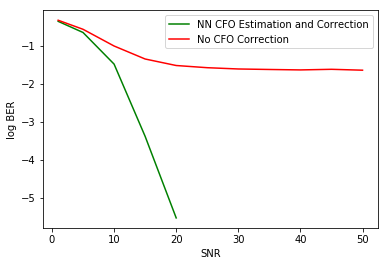
\includegraphics[width=12cm]{figures/cfo/cfo_estimation.png}
\caption{The log BER of received signals passed through a neural network CFO estimator with a rotation matrix CFO correction and classic demodulator. The log BER of the same signals passed through just the classic demodulator.}
\label{fig:cfo_est}
\end{center}
\end{figure}

For SNR above $25$, the neural network does not have any incorrect bits in the $10k$ data sequences each with $100$ symbols, or $200$ bits.  The neural network consistently performs better than just the classic demodulator for all SNR.  Although, the performance is similar for SNR$=1$.
Figure~\ref{fig:cfo_demon_single_tap} shows one example of a data sequence passed through the neural network described above.
The neural network is trained for SNR$=\infty$ with the same training sequence as described above. The estimated data constellation plot has removed most of the effects of the CFO and looks quite similar to the original data constellation plot.

\setlength{\tabcolsep}{0pt}
\begin{figure}
  \centering
  \caption{Nonlinear neural network estimating and correcting CFO for different $\omega$. In this particular test example, $\omega=0.00969545$ and SNR$=\infty$. The figure on the left shows the constellation of the $100$ original data symbols. The figure in the middle shows the constellation of the original data symbols after CFO. The figure on the right shows the constellation of the data symbols after the neural network CFO correction.}
  \begin{tabular}{ccc}
    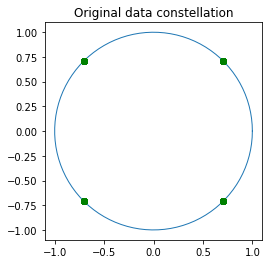
\includegraphics[width=55mm]{figures/cfo/cfo_estimation_original_data.png}&
    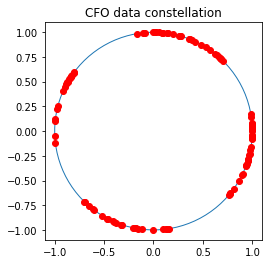
\includegraphics[width=55mm]{figures/cfo/cfo_estimation_cfo_data.png}&
    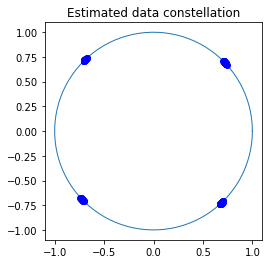
\includegraphics[width=55mm]{figures/cfo/cfo_estimation_est_data.png}\\
  \end{tabular}
  \label{fig:cfo_demon_single_tap}
\end{figure}

In this chapter, we demonstrated that recursive neural networks can act like clocks; they can follow a circle for a given rate of rotation.  They can learn to learn to follow a circle for a given rate.
We have also demonstrated that a neural network can learn to learn how to estimate CFO and correct for it.  All of the simulations in this chapter were for single tap channels.  We attempted to learn how to estimate CFO and correct for it when there were random two tap channels.  However, the results were not promising and will need to be explored more in future work.

%\section{Deep Network Carrier Frequency Offset Correction}
%Program a Costas loop for comparison 

\section{Future Work}

In addition to the future work described in Chapter 2, we want to expand our CFO estimation and correction work.
We want to estimate CFO even in the presence of mullti-tap channels and when the channels have complex taps.
We also want to explore replacing the rotation layer that does the CFO correction with the RNN that follows a circle.  Then the entire process will be based in neural networks without much structure.
We also want to combine all of the aspects in this report to create one deep equalizer network that corrects for CFO and equalizes the channel.  We may not explicitly need networks that do the estimation but it is a good place to start.

In general, this report was more of an exploration into how neural networks can learn to learn to communicate for equalization and CFO correction.  We would like to do a more thorough architecture search and longer training runs.  We also hope to to verify the ideas presented in this report by training on real radio data instead of simulated data.
\chapter{Conclusion}

In this report, we reviewed the current literature on machine learning systems for communcations systems; specifically equalization and carrier frequency offset.  We also discussed the value of robustness and adaptability in future communications systems requiring an investigation of meta-learning.
We demonstrated that neural networks can learn to learn to estimate channel characteristics for two tap channels.  We explored using deep recursive neural networks to learn to learn to equalize.
We also used recursive neural networks to learn to learn to be a clock by rotating in a circle at different rates.  Lastly, we used deep neural networks to estimate the rate of carrier frequency offset and correct it.

All of this was achieved without using backpropagation when faced with new environments.
From here, we plan to continue developing our work and design an end-to-end receiver, including demodulation and error correction, in neural networks that can adapt to new multipath channels and carrier frequency offsets. 
Communications is a perfect application to explore the possibilities and limitations of the current meta-learning and machine learning frameworks.  


% \appendix
% \chapter{More Monticello Candidates}

\printbibliography

\end{document}
